\documentclass[11.5pt]{sig-alternate} % sets document style to sig-alternate
% packages
% typesetting
% \usepackage{dirtytalk} % can be used to typset quotes easier, automatically sets correct quotation marks with \say{content}
% \usepackage{hanging} % hanging paragraphs with \hanging, like in references. doesn't translate to HTML
\usepackage[defaultlines=3,all]{nowidow} % avoid widows
\usepackage[pdfpagelabels=false]{hyperref} % produce hypertext links, includes backref and nameref
\usepackage{xurl} % defines url linebreaks, loads url package
\usepackage{microtype} % better typography
% layout
\usepackage{calc} % so we can do inline math within \setlength
% \usepackage{enumitem} % control layout of itemize, enumerate, description
\usepackage{fancyhdr} % control page headers and footers
% \usepackage{float} % improved interface for floating objects, adds H float
% \usepackage{multicol} % intermix single and multiple column pages
% \textgreek % typeset greek letters in text mode
% language
\usepackage[utf8]{inputenc} % utf8 encoding, wider character set
\usepackage[english]{babel} % multilanguage support
% misc
\usepackage{graphicx} % builds upon graphics package, \includegraphics
%\usepackage{lastpage} % reference number of pages
\usepackage{xcolor} % color extensions
\usepackage[backend=biber, style=apa]{biblatex} % sophisticated bibliographies % necessary for HTML to display author info and date on abstract page
\usepackage{csquotes} % advanced quotations, makes biblatex happy
\usepackage{authblk} % support for footnote style author/affiliation
% tables and figures
%\usepackage{array} % extend array and tabular environments
\usepackage{caption} % customize captions in figures and tables (rotating captions, sideways captions, etc)
%\usepackage{cuted} % allow mixing of \onecolumn and \twocolumn on same page
\usepackage{multirow} % create tabular cells spanning multiple rows
%\usepackage{subfigure} % deprecated, support for manipulation of small figures
\usepackage{tabularray} % better table construction, does not translate to HTML
%\usepackage{wrapfig} % allows figures or tables to have text wrapped around them
% dummy text
%\usepackage{blindtext} % blind text dummy text
%\usepackage{kantlipsum} % Kant style dummy text
\usepackage{lipsum} % lorem ipsum dummy text

\pagestyle{fancy} % sets pagestyle to fancy for fancy headers and footers
% allows the header to take the full width of the page https://www.reddit.com/r/LaTeX/comments/awtrb2/how_to_you_make_the_headerfooter_extend_the/
\newlength{\oddmarginwidth}
\setlength{\oddmarginwidth}{1in+\hoffset+\oddsidemargin}
\newlength{\evenmarginwidth}
\setlength{\evenmarginwidth}{\evensidemargin+1in}
\fancyhfoffset[LO,RE]{\oddmarginwidth}
\fancyhfoffset[LE,RO]{\evenmarginwidth}

% header and footer
% modern way to set header image
\renewcommand{\headrulewidth}{0pt} % defines thickness of line under header
\renewcommand{\footrulewidth}{0pt} % defines thickness of line above header
\setlength\headheight{80.0pt} % sets height between top margin and header image, effectively moves page contents down
\addtolength{\textheight}{-80.0pt} % seems to affect the lower height. maybe only works properly if footer numbers enabled?
\fancyhf{}
\fancyhead[CE, CO]{
\includegraphics[width=\pdfpagewidth]{headerImage.png}}

\hypersetup{colorlinks=true,urlcolor=blue} % sets link color to blue
\urlstyle{same} % sets url typeface to same as rest of text

% set caption and figure to italics, label bold, left align captions, does not transfer to HTML
\captionsetup{labelfont=bf, font={large, it}, justification=raggedright, singlelinecheck=false}
\renewcommand\theContinuedFloat{\alph{ContinuedFloat}} % has something to do with subfigures... don't remember why i used it

%this next bit is confusing, but essentially changes the width of the abstract. Seems to have been copied from this https://tex.stackexchange.com/questions/151583/how-to-adjust-the-width-of-abstract
\let\oldabstract\abstract
\let\oldendabstract\endabstract
\makeatletter %changes @ catcode to enable modification (in parsep)
\renewenvironment{abstract} %alters the abstract environment
{\renewenvironment{quotation}%
               {\list{}{\addtolength{\leftmargin}{1em} % change this value to add or remove length to the the default ?
                        \listparindent 1.5em%
                        \itemindent    \listparindent%
                        \rightmargin   \leftmargin%
                        \parsep        \z@ \@plus\p@}%
                \item\relax}%
               {\endlist}%
\oldabstract}
{\oldendabstract}
\makeatother %changes @ catcode to disable modification

% checks
% italics 
% links
% dashes
% tildes
\begin{document}
\title{Making Science-Inquiry Learning Accessible \\ for Students with Complex Support Needs}

\author[1]{\large \color{blue} Sarah Koebley} % make sure there are no spaces after the author's name
\author[2]{\large \color{blue} Shawnee Wakeman}
\author[1]{\large \color{blue} Lindsay Ruhter}
\author[2]{\large \color{blue} David Pugalee}
\author[1]{\large \color{blue} Meagan Karvonen}

\affil[1]{University of Kansas, Accessible Teaching, Learning, and Assessment Systems (ATLAS)}
\affil[2]{University of North Carolina at Charlotte}
\toappear{} % the sig.alternate document type includes a copyright warning that appears at the bottom of the first page. This makes that not appear/be empty. Don't ask my why it's there in the first place /shrug

\maketitle % prints article title
\begin{@twocolumnfalse} 
\begin{abstract}
\item %the abstract is a quotation and a list, so this must be an item
\begin{large}
\textit{Inquiry learning through engagement with scientific practices has proven to be an effective instructional practice for general education students. Although students with complex support needs (CSN) are required to have access to the same grade-appropriate academic content in science as their peers without CSN, it remains a challenge for special education teachers to design instruction around student inquiry and science conceptual understanding. The 5E Science Education for Special Educators (5E-SESE) Model combines three well-established conceptual constructs (three-dimensional science standards, Universal Design for Learning [UDL], and the 5E Model) to support special educators in delivering quality science instruction. With the 5E Model at its center, 5E-SESE emphasizes the importance of students with CSN as active learners engaged in science practices. Three-dimensional content standards supported by UDL ensure rigor and accessibility for all students. This paper describes 5E-SESE and how it supports teachers’ design of effective science-inquiry instruction for students with CSN.}
\item Keywords: inquiry, universal design, multidimensional science, special education, students with disabilities, extensive support needs, complex support needs

\end{large}     
\end{abstract}
\end{@twocolumnfalse}

%% AUTHOR INFORMATION
\textbf{*Corresponding Author, Sarah Koebley}\\ % corresponding author
\href{mailto:koebleys@ku.edu}{(koebleys@ku.edu)} \\ % author email
\textit{Submitted Apr 5 2023} \\ % submitted date
\textit{Accepted May 14 2024} \\ % accepted date
\textit{Published Online Jan 21 2025} \\ %published online date, updated after author approval
\textit{DOI: 10.14448/jsesd.16.0005} \\ % doi, updated after author approval, in spreadsheet on server
\pagebreak 
\clearpage %both needed to go to next page
\begin{large}
\section*{INTRODUCTION}
For several decades, reform in science education has advocated for student inquiry in science classrooms (National Research Council [NRC], 2000, 2012). For students to fully understand scientific concepts, they must participate in the inquiry processes and discourse by which those science and engineering ideas were developed (NRC, 2012). These recommendations, along with the requirement that all students have access to the general education curriculum (Individuals With Disabilities Act [IDEA], 2004), have prompted a shift in instruction for students with complex support needs\footnote{Students with complex support needs (CSN) comprise about 9\% of the population of students with disabilities, or about 1\% of the overall student population. We recognize and build on research for this population that includes students with severe intellectual disability, significant cognitive disabilities, extensive support needs, autism, or multiple disabilities. In this paper, students with CSN includes all students with disabilities that significantly impact their intellectual functioning and adaptive behavior (Nash \& Bechard, 2016).} (CSN), that is, the approximately 1\% of students for whom general, statewide assessments with accommodations do not produce valid evidence of what those students know and can do. For science instruction, inquiry learning through engagement with scientific practices is recommended as a primary strategy for general education students (Minner et al., 2010; Osborne, 2014), as well as for those with disabilities (Rizzo \& Taylor, 2016). What implications might the call for science-inquiry learning have for students with CSN and the teachers who support them?

\textit{Inquiry} is defined as learners asking important questions about the natural and designed world, gathering evidence to answer those questions through investigation, and then communicating their findings using that evidence (NRC, 2000). An effective approach to learning, inquiry science is also critical in developing citizens who are informed decision makers (Tan et al., 2023). However, scientific inquiry for students with CSN has been more difficult to define and operationalize. It remains a challenge for teachers to provide their students with CSN the required access to the same grade-appropriate academic content in science, including inquiry instruction, that is accessed by their peers in general education (Kuntz \& Carter, 2019; Petersen, 2016). This challenge exists in part due to the different theories of science learning that have guided reform in special education and general education classrooms (Taylor et al., 2020). 

This paper, building on recent promising results in the use of inquiry with students with CSN (Jimenez et al., 2021; Knight et al., 2020) and on robust findings of the use of learning-cycle models with general education students (Minner et al., 2010; Taylor et al., 2015), introduces a model for teachers of students with CSN that situates student inquiry and science conceptual understanding at its center. We describe the three conceptual constructs that comprise the 5E Science Education for Special Educators (5E-SESE) Model, the rationale for their inclusion, and how the model supports special educators in their design of quality science instruction for students with CSN.\footnote{5E-SESE is a professional development project that uses the same 3-construct model to both guide teacher learning and support student inquiry. This paper focuses on how the model supports student inquiry. See Karvonen et al., 2024 for a description of the 5E-SESE professional development approach.}

\section*{BACKGROUND: SCIENCE INSTRUCTION \\FOR STUDENTS WITH COMPLEX \\SUPPORT NEEDS}

In the years following IDEA (2004), reforms aimed at providing access to the general education curriculum for students with CSN typically targeted the skills needed to support learning in functional life-skills domains (Browder et al., 2004). Legislation (Every Student Succeeds Act, 2015) requires that content standards for assessments for students with CSN be based on alternate achievement standards that align with the grade-level content standards for all students. Enacted curriculum studies in the years following passage of the legislation, however, indicated that teacher expectations for students’ learning were limited, often resulting in science instruction that was not age appropriate (Karvonen et al., 2013) and focused primarily on skills needed for daily living rather than on more rigorous academics.

While there have been increasing calls for students with CSN to be able to use science practices to demonstrate understanding of science concepts (Andersen \& Nash, 2016), an ongoing divide exists between the underlying theories of science learning in special education and those in general education. Sociocultural and cognitive models emphasize learning that occurs in a social context (e.g., inclusion models, incorporating students’ environments and interests) that encourages students to construct meaning for themselves (including through methods such as inquiry). These models undergird inquiry-based methodologies that led to science reform within general education (McGinnis \& Kahn, 2014). Yet, special education research has been dominated by behaviorist-oriented studies that define learning in terms of student mastery of specific skills and information (McGinnis \& Kahn, 2014). While inquiry instruction remains the gold standard for science instruction in general education classrooms (Osborne, 2014), students with disabilities, who typically require more structured learning environments, learn science concepts most often through direct and explicit instruction (Rizzo \& Taylor, 2016).

Although shifts towards an academic focus have occurred recently for students with CSN (Spooner \& Browder, 2015), science instruction has typically been either embedded within functional-curriculum objectives (e.g., making decisions about safety, health, and nutrition in daily activities) or implemented using explicit systematic instruction to elicit desired student responses for the measurable outcomes being targeted (e.g., recall of vocabulary, successful completion of steps to conduct an experiment) (Spooner et al., 2011). 

Recent studies report evidence of improved achievement for students with disabilities (including students with intellectual disabilities and Autism Spectrum Disorder [ASD]) when inquiry instruction was implemented (Rizzo \& Taylor, 2016). Instruction informed by inquiry approaches such as use of the scientific method or a learning cycle (Bybee et al., 2006) were effective for students with disabilities when they were implemented with some components of explicit instruction (Rizzo \& Taylor, 2016). Similarly, a review of adjacent literature on science instruction for students with ASD (where inquiry included student observation, experimentation, and reasoning) found that students benefitted from the use of inquiry methods (e.g., hands-on exploration) and with support using direct instruction (Barnett et al., 2018).

Knight et al. (2020) summarized research focused on learning both science content and science practices for students with intellectual disabilities and ASD (students with CSN represented a subset of those students included within studies in the review). They found that use of science practices led to increased student ability to generalize certain science concepts (e.g., living things are alive). Students with CSN have also been able to successfully engage in inquiry by asking more in-depth questions in science units focused on developing engineering habits of mind (Jimenez et al., 2021). Universal Design for Learning (UDL) principles provided the construct needed for the teachers in this study to reduce barriers and increase access to inquiry for this population of students.

Although Apanasionok et al.’s (2019) recent literature review reported that a preponderance of evidence supports behavioral approaches (e.g., systematic instruction) in science as effective for students with CSN, the study’s authors acknowledge that the dominant paradigm in U.S. special education research has been conducted within a dedicated but small research community. These studies and others (Taylor et al., 2020) call for broader definitions of effective science instruction for students with CSN that allow for inclusion of a wider range of strategies, including strategies (like inquiry-oriented approaches and UDL-focused adaptations) that have been used successfully in general education classrooms.

\section*{PREPARING SPECIAL EDUCATION TEACHERS FOR A NEW MODEL IN SCIENCE INSTRUCTION}

Students with CSN are most often taught in segregated settings (Andersen \& Nash, 2016) by special educators who do not have licensure or extensive preservice training in science academic content (Osborne, 2014). Given the shifts toward more inquiry-focused academic instruction, special educators are required to fulfill increasingly complex roles in service of students with CSN. While most preservice special educator programs include a focus on specially designed instruction with adaptations and supports, the planning of inquiry-based instruction using newer multidimensional standards and UDL is likely neither included nor intuitive (van Garderen et al., 2020). When academic-content-area coursework is included, it is more likely to address literacy and numeracy content than science concepts (Leko et al., 2015). While alternate science-content standards outlining grade-appropriate academic content for students with CSN have been written, designing inquiry-oriented instruction using those standards is challenging to implement (Petersen, 2016).

Special education teachers, all of whom have varying preparation levels and experiences, need to design and deliver specialized instruction to address diverse learning goals (e.g., priority goals of communication, social skills, life skills) balanced with required academic content for students with CSN (Root et al., 2017). These complexities present a challenge to teachers as they align individual student needs with instructional priorities, especially given limited instructional time.

This paper introduces a model that supports inquiry science instruction of students with CSN. The 5E-SESE Model supports teachers in applying inquiry-based teaching strategies to robust science content with their students (Karvonen et al., 2024). While other recent studies have proposed inquiry learning as an organizing principle for multiple constructs (Molebash et al., 2019), the 5E-SESE Model defines an inquiry-oriented organization of components inclusive of UDL-focused instruction for students with CSN. We describe how the component parts of each of the three conceptual constructs support inquiry learning for students with CSN and provide an example of how teachers have used the model to guide their design of inquiry-oriented science instruction.

\section*{A CONCEPTUAL MODEL: SCIENCE-INQUIRY INSTRUCTION FOR STUDENTS WITH CSN}

The 5E-SESE Model builds teacher knowledge of inquiry instruction for students with CSN, continuing a shift toward strategies that prioritize student conceptual understanding in science. This model builds on studies that use UDL principles to support inquiry-based science instruction for students with and without disabilities (Hanuscin \& van Garderen, 2020; Sebti \& Damiani, 2021).

The 5E-SESE Model (Figure 1) situates the 5E Instructional Model at its center to emphasize the focus on inquiry, with students as active participants in scientific processes. The 5E Instructional Model (Bybee, 2014) consists of five instructional phases (Engage, Explore, Explain, Elaborate, and Evaluate) that form a learning cycle. While multidimensional standards guide the concepts and skills to include in science instruction, the 5E model provides a structure for how learners can engage deeply with that content. With a substantial body of evidence showing that inquiry-based instructional strategies increase students’ conceptual understanding of science ideas (Minner et al., 2010), models like the 5E model provide a foundation and a starting place for shifts toward instruction that expect active student thinking and engagement.

\begin{figure}[htb]
    \centering
    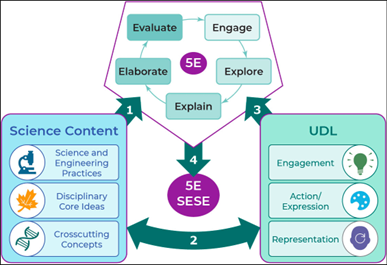
\includegraphics[width=\columnwidth]{images/fig1.png}
    \caption{5E-Science Education for Special Educators (5E-SESE) Model}
    \label{Figure 1}
\end{figure}

Within the 5E-SESE Model, the 5E inquiry cycle is supported by three-dimensional science content standards (Figure 1, Arrow 1). Including standards with a full slate of core content, science practices, and crosscutting concepts assures that students with CSN are offered access to the same rigorous standards as their general education peers. The standards also offer extensive opportunities for student engagement as they connect science learning with experiences of their immediate surroundings and personal space (Bybee, 2014).

UDL principles also support the 5E inquiry cycle (Figure 1, Arrow 3), providing guidelines to identify barriers and design solutions during instruction. Both constructs emphasize student engagement; the Engage 5E phase uses students’ interests and prior knowledge as a first step in inquiry. The UDL engagement principle recognizes that not all students approach learning in the same way, supporting early identification of potential barriers in instructional planning with the ultimate goal of providing diverse means for students to interact with content, their peers, and their teachers (Israel et al., 2018; Thomas et al., 2018). Similar mutual connections occur between the other phases of the 5E model and the UDL guidelines of Action/Expression and Representation (e.g., identifying alternate ways to communicate findings in an Explain phase, including additional methods for gathering data in an Explore phase). Using different combinations of the constructs’ component parts in this way demonstrates the multiple ways inquiry can be enacted (connecting different elements of UDL and the 5E model) as opposed to defining one single correct approach.

Three-dimensional science-content standards and UDL also have complementary components that support the 5E inquiry cycle (Figure 1, Arrow 2). UDL guidelines for creating engaging and accessible learning experiences (CAST, 2018) align with the science practices’ emphasis on the use of scientific models, investigations, and discourse about ideas (Summy \& Fetters, 2018). The crosscutting concepts’ (CCCs) progression of major conceptual ideas supports the UDL principle of providing multiple means of representation through encouraging use of graphic organizers, assistive technology, or scaffolding. The CCCs also give students broad categories around which to ask questions and convey their knowledge using UDL-based approaches like explicit strategy teaching, thus providing multiple means of action and expression (Hebert et al., 2018).

The 5E-SESE Model integrates three well-re\-searched constructs that support teachers in designing effective instruction. The 5E model, supported by robust science content and UDL-based adaptations that reduce learning barriers, defines 5E-SESE (Figure 1, Arrow 4). Each of the three constructs is described in more detail in the sections that follow.

\subsection*{Multidimensional Science Standards for All}

A vision of science learning is outlined in the Framework for K–12 Science Education (NRC, 2012) and the Next Generation Science Standards it supports (NGSS, 2013) wherein all students learn fundamental scientific concepts through the integration of science practices and crosscutting themes. This innovative three-di\-mensional model uses the following guidelines to define standards and learning expectations:

\begin{itemize}
    \item \textit{Science and engineering practices} (SEPs) develop students’ thinking around real-world challenges and contexts; they provide an opportunity for students to apply knowledge in ways that reflect the kinds of thinking and practices that scientists and engineers engage in while developing theories and models, designing solutions, and communicating new findings (Brand, 2020).
    \item \textit{Disciplinary core ideas} (DCIs) are the key science concepts, defined across multiple science domains, that progress within and across grade levels to build understanding of complex ideas and connect to students’ interests and life experiences (NRC, 2012).
    \item \textit{Crosscutting concepts} (CCCs) are broad themes that organize conceptual development across the DCIs and SEPs. They include patterns, similarity, and diversity; cause and effect; scale, proportion, and quantity; systems and system models; energy and matter; structure and function; and stability and change (NRC, 2012).
\end{itemize}

The three dimensions provide structure for students as they investigate questions about the natural world and define and explore engineering design challenges.

With states’ adoption of these multidimensional science standards, learning expectations for all students, including students with CSN, shifted. For example, Essential Elements (EEs) are extended science content standards (Dynamic Learning Maps Consortium [DLM], 2017) used in more than 20 states. These standards support grade-banded performance expectations in reduced depth and complexity to assure that important and rigorous science content is accessible to students with CSN (Nash \& Bechard, 2016). Like the NGSS performance expectations, each EE is defined in terms of the aligned DCIs, SEPs, and CCCs (Table 1). 

\begin{table*}[thbp]
\caption{Examples of How Next Generation Science Standards Were Adapted to Develop Dynamic Learning Maps (DLM) Essential Elements}
\begin{tabular}{|l|l|}
\hline
Next Generation Science Standard & DLM Essential Element \\ \hline
5-ESS3-1: Obtain and combine information about ways individual communities use science ideas to protect the Earth’s resources and environment. & EE.5-ESS3-1: Use information to describe how people can protect the Earth’s resources and how that affects the environment. \\ \hline
MS-PS3-5: Construct, use, and present arguments to support the claim that when the kinetic energy of an object changes, energy is transferred to or from the object. & EE.MS-PS3-5: Support an argument with evidence that when the kinetic energy of an object changes, energy is transferred to or from the object. \\ \hline
HS-ETS1-4: Evaluate a solution to a complex real-world problem based on prioritized criteria and trade-offs that account for a range of constraints, including cost, safety, reliability, and aesthetics as well as possible social, cultural, and environmental impacts. & EE.HS-ETS1-4: Evaluate a solution to a real-world problem that accounts for technical constraints as well as community impacts. \\ \hline
\end{tabular}
\end{table*}

Within the DLM Assessment System, EEs specify grade-level learning targets, and learning maps clarify how students can reach those learning targets. For each EE, the learning map defines a path toward the EE’s learning target(s) using nodes that reduce complexity even further. These nodes, called linkage levels, give students an opportunity to grow toward the learning targets of grade-level general education content standards (Dynamic Learning Maps, 2017). 

Science EEs raise the bar for what can be expected of students with CSN in terms of conceptual knowledge acquisition and cognitive complexity. Application of SEPs and CCCs allow students to demonstrate understanding of science concepts and make connections with other literacy or content-area practice standards (Houseal et al., 2016).

\subsection*{Universally Designed Science Instruction}

UDL, in support of inquiry learning, is an essential component of the 5E-SESE Model. The goal of UDL is to “develop expert learners who are, each in their own way, resourceful and knowledgeable, strategic and goal-directed, purposeful and motivated” (CAST, 2018, FAQ section, para. 1). UDL addresses this goal through three principles that support the design of the most accessible experience or content for learners. The principles are organized into guidelines to articulate further the why, what, and how of learning, as well as strategies for students to access, build, and internalize the learning (CAST, 2018). Each guideline is further divided into checkpoints that suggest how teachers can teach that guideline. The checkpoints are not exhaustive; rather, they are ideas, plans, or actions that serve as a basis for developing learning options and supports for all students.

The first UDL principle articulates strategies to assure that all students are engaged with learning and includes three guidelines: recruiting interest, sustaining effort and persistence, and self-regulation. Providing multiple means of representation for all learners is the second UDL principle and includes the guidelines of perception, language and symbols, and comprehension. Finally, the third principle describes multiple means of action and expression for learners to show what they know and can do and includes options for physical action, expression and communication, and executive functions.

UDL principles and guidelines can support science learning through hands-on investigations, scientific discourse, and community-based instruction (Hebert et al., 2018; Summy \& Fetters, 2018); they also can create accessible learning opportunities for all students, with and without disabilities, increasing opportunities for scaffolding and reducing barriers to learning. Recent studies have shown promise using universally designed engineering instruction for students with CSN. Researchers used UDL principles to adapt a high-quality, general-education engineering curriculum for students with CSN. Setting self-determination goals involving initiation, thinking, and collaboration; students’ ability to ask substantial questions improved over the course of the study (Jimenez et al., 2021). UDL has also been used to mediate the significant language demands of learning science for students with disabilities (Thomas et al., 2018) and in teaching engineering concepts to students with ASD (Kouo et al., 2021).

\subsection*{5Es for Inquiry-Based Instruction}

The 5E-SESE Model is based on learning theory which holds that people reinterpret, redefine, reorganize, elaborate, and change conceptual understanding as they interact with their surroundings (Bybee et al., 2006). By interpreting phenomena through the lens of their experiences, learners develop the knowledge and expertise necessary for them to understand and engage with the world around them (NRC, 2012).

5E-SESE incorporates a five-phase learning cycle structure: \textit{Engage}, \textit{Explore}, \textit{Explain}, \textit{Elaborate}, and \textit{Evaluate}. Each phase has a specific function that supports inquiry instruction. In the Engage phase, teachers motivate students to want to learn about a topic, while also learning what students already know about the topic. Students pose questions about phenomena in which they have interest. During the Explore phase, students participate in hands-on activities to observe a phenomenon, collect data, and test out varying designs or variables. Data is analyzed and scientific vocabulary is used to describe findings and make claims during the Explain phase. In the Elaborate phase, students ask related questions or apply their learning about a science concept to another context. Finally, student understanding is assessed during the Evaluate phase. Teachers enable and guide inquiry throughout all five phases, offering varying levels of guidance as students gain understanding and construct meaning for themselves (Bybee, 2014). 

Studies of the 5E model indicate many positive effects on student learning and increasing student interest in science (Bybee et al., 2006; Bybee, 2014; Minner et al., 2010). 5E instruction challenges students’ existing understandings and knowledge, allows for the reconstruction of false assumptions (Bybee, 2014; Ruiz-Martín \& Bybee, 2022), and promotes deep learning that is grounded in students’ personal experiences (Concannon \& Brown, 2017).

The model requires adaptation to support conceptual learning for students with CSN. Several studies have found that explicit instruction embedded within a guided-inquiry approach increased students’ science learning outcomes, including in students with learning disabilities (Rizzo \& Taylor, 2016). Instructional approaches of this type represent a shift in thinking about how students with disabilities learn and how they can be expected to engage with academic content. Successful use of instructional strategies—like guided inquiry with hands-on activities, spatial organizers, peer mediation, and formative feedback (Therrien et al., 2014; Toma, 2022)—have expanded special education research beyond the well-established literature on behavior\-ist-focused instruction.

Some aspects of the 5E-SESE Model are supported for instruction of students with disabilities (Sebti \& Damiani, 2021; van Garderen et al., 2020). In literacy, for example, approaches in science writing have been shown to be effective in providing access to argument-based science inquiry for students with disabilities (Taylor et al., 2018). Students with moderate- to severe-intellectual disabilities were able to ask scientific questions, make observations, design and carry out investigations, and draw conclusions using electronic devices in an adapted 5E approach (Miller et al., 2013). Likewise, So et al.’s (2022) adapted 5E instructional model allowed students with mild to moderate intellectual disabilities to actively engage with STEM learning through technology exploration, explaining for understanding, and engineering innovation.

While inquiry instruction is a common strategy for science, it is not often used when teaching students with CSN. Teachers must have knowledge of science content and of how to engage students with disabilities effectively with these concepts, as well as tools for addressing the barriers their students will face in inquiry-oriented instruction (Israel et al., 2018). Using the 5E-SESE Model, special education research can be expanded to focus on how to apply UDL-infused science-inquiry methodologies with students who have CSN.

\section*{IMPLEMENTING THE 5E-SESE MODEL}

The 5E-SESE Model operationalizes the three constructs described above for instruction in science content (rigorous three-dimensional standards), inquiry-based science teaching pedagogy (the 5E model), and ensuring accessibility for all learners (UDL). Ultimately, the goal of inquiry-focused instruction is for students with CSN to be able to construct meaning and communicate about solutions to authentic problems (Kouo et al., 2021) as they develop increased autonomy, capacity for self-advocacy, and human connection (Erickson \& Koppenhaver, 2020). How does the 5E-SESE Model support teachers’ design of effective science-inquiry instruction for students with CSN?

\subsection*{Teacher Design of Instruction Guided by the 5E-SESE Model}

The 5E-SESE Model is based on the philosophy that a UDL-supported 5E approach to inquiry teaching and learning is an effective organizer for special educators’ design and planning of science instruction. The convergence points of the three constructs represent opportunities for teachers to think about science instruction in innovative ways. For example, cognitive themes (e.g., cause and effect, patterns, change over time) and science practices (e.g., questioning, investigating, modeling) represented by dimensions in the science standards increase options for access and engagement for students with CSN (Figure 1, Arrow 2). Similarly, the UDL guidelines are themselves a starting point for planning instruction that is accessible, engaging, and challenging (Ruhter, 2022). There is great benefit in designing instruction that addresses learning variability from the onset rather than retrofitting adaptations for specific learners into developed lessons, particularly in the context of science-lesson planning for students with CSN (Jimenez, 2020).

\begin{table*}[thb]
\caption{5E-SESE Model Aligned to 5E-SESE Lesson Planning Steps}
\begin{tabular}{|l|l|l|}
\hline
5E-SESE Model Component & Teachers’ Planning Decisions & 5E-SESE Lesson Planning Steps \\ \hline
Science Content: Three-Dimensional Science Standards & Teachers learn each dimension for the standard and the aligned Essential Element (EE); teachers begin to consider opportunities to extend themes across content areas and identify where students focus their science learning on the basis of the chosen EE. & \begin{tabular}[x]{@{}l@{}} Based on EE chosen: \\1. Identify Science and Engineering Practice \\ 2. Identify Disciplinary Core Idea \\ 3. Identify Crosscutting Concept \\ 4. Identify linkage levels (content that builds to and supports the target EE) \end{tabular} \\ \hline
Universal Design for Learning (UDL)	& \begin{tabular}[x]{@{}l@{}} Teachers choose UDL options based on general accessibility considerations and specific support needs for this science lesson; teachers write ideas for engagement according to student interests and prior learning. \\ Based on the EE, teachers choose a science topic where students have interest or previous experience, and then identify common student misconceptions about that topic; teachers identify specific science content that may indicate barriers to student learning; teachers write strategies that mitigate or avoid barriers. \end{tabular} & \begin{tabular}[x]{@{}l@{}} 5. Identify student’s UDL accessibility supports \\ 6. Identify student’s prior experiences and prior knowledge \\ 7. Choose science phenomenon of interest for lesson focus \\ 8. Identify common student alternative conceptions \\ 9. Identify specific barriers and UDL solutions \end{tabular} \\ \hline
5E Model & Teachers use this information, using the 5E steps to design a lesson for students with CSN that progresses from engagement to evaluation. & \begin{tabular}[x]{@{}l@{}} Identify teacher and student actions to: \\ 10. Engage \\ 11. Explore \\ 12. Explain \\ 13. Elaborate \\ 14. Evaluate \end{tabular} \\ \hline
\end{tabular}
\end{table*}

Each component of the 5E-SESE Model supports teachers’ instructional decision-making (Table 2). A “Lesson Planning Fundamentals” module and a lesson plan template, both aligned to the 5E-SESE Model, are designed to support teachers throughout the planning process. To help teachers learn three-dimensional science content, identify and use UDL strategies, and employ the 5E model when creating inquiry lessons, we created an online course based on the 5E-SESE Model. The course includes a step-by-step lesson-planning approach to assist teachers in creating instruction that is tailored to student strengths, interests, and needs (Karvonen et al., 2024). The 5E lesson plan itself serves as a graphic organizer to ensure that instructional planning begins with identifying and understanding the SEP, DCI, and CCC associated with a teacher-selected EE.

% table 2 original position

As they identify ways to engage learners in EE-specific science content, teachers are prompted to note students’ prior experiences and general accessibility needs. Teachers choose scientific phenomena that allow students to experience cognitive challenges and strategy development by considering student interests and preferences, communication skills, and self-determination abilities. Next, barriers specific to learning the chosen science phenomenon are listed so that UDL adaptations can be identified to keep students actively engaged, both mentally and physically (Figure 1, Arrow 2). Finally, guidance through phases of the 5E model supports teachers in their decisions as they select, sequence, and assess learning activities.

The 5E-SESE Model in action provides an example: 

\begin{quote}
A middle school special education teacher is designing a lesson about chemical changes for her students with CSN. She begins by identifying the SEP (analyzing and interpreting data), DCI (substances react chemically in characteristic ways), and CCC (use patterns to identify cause and effect and use graphs of data to identify patterns) from the standard. She then considers her students’ existing knowledge to ensure accessibility (e.g., graphic organizers, vocabulary reference page) and build on prior experiences (e.g., can identify change, temperature, texture, and states of matter). She decides to build the lesson around the phenomenon of how pennies change color when a chemical reaction occurs. For \textit{Engage}, she includes objects for students to interact with (e.g., wood and burnt wood, pennies, bread and dough), making sure to program student communication devices with appropriate vocabulary and sentence stems that support student responses to questions posed. For \textit{Explore}, the teacher uses videos, objects, and a graphic organizer (data table) so students can observe and record data about common substances before and after chemical changes occur. In \textit{Explain}, the teacher will have students complete a structured scientific response to have them use their data and vocabulary to answer the investigation’s question. An \textit{Elaborate} phase includes additional investigations (with different objects) to allow students to gather more data that verifies initial findings about the properties of chemical changes. \textit{Evaluation} occurs throughout the cycle as teachers gather evidence of learning and in a final summative assessment that asks students to identify chemical changes using vocabulary learned in the lesson.
\end{quote}

Teachers participating in the 5E-SESE project receive virtual professional-development (seven learning modules and an online lesson plan tool) and one-on-one coaching (throughout the planning cycle and in analysis of videotape of the enacted lesson) as they design and deliver inquiry-based science instruction to students with CSN (Karvonen et al., 2024).

\section*{CONCLUSION}

Using science content from the three dimensions represented in the K–12 Science Framework, the 5E-SESE Model is designed to support a new approach to science instruction for students with CSN. With inquiry at the center of the model in the form of the 5Es, teachers are supported as they design robust science instruction supported by UDL principles. Our work builds on promising results in the use of inquiry with students with disabilities (Jimenez et al., 2021; So et al., 2022) and extends prior research integrating 5E, UDL, and formative assessment approaches (van Garderen et al., 2020) to provide a model specifically aimed at supporting teachers in designing science-inquiry instruction for students with CSN. The model also builds on studies that shift emphasis for students with CSN from skill-based science instruction to strategies aimed at students’ conceptual understanding (Jimenez et al., 2021; Knight et al., 2020).

The project supports the use of robust science standards and inquiry instruction that benefit not only students with CSN but also likely will provide more-accessible strategies for all learners (Rose et al., 2005; Thomas et al., 2018), including those who are underrepresented in STEM professions (Clements et al., 2021). Natural overlaps between the NGSS and UDL provide opportunities for underserved populations to have increased access to rigorous science coursework, regardless of differences in culture, language, or academic ability (Rudenstine et al., 2018).

As more learning opportunities for students with CSN are envisioned and carried out successfully, the shift in classroom and research emphasis from skill-oriented instruction to strategies involving inquiry and conceptual understanding becomes more viable. With research continuing to bolster the learning theories behind the three constructs in our model, this project outlines an approach to science instruction that serves the unique learning needs of students with CSN.

\section*{AUTHOR NOTE}

The research reported here was supported by the Institute of Education Sciences, U.S. Department of Education, through Grant R324A180202 to the University of Kansas Center for Research with Institutional Review Board approval (142906). The opinions expressed are those of the authors and do not represent views of the Institute or the U.S. Department of Education. The authors report no competing interests to declare.

The authors wish to thank Lori Andersen for her contributions to initial conceptualizations of an approach that supports science-inquiry for students with complex support needs.

Correspondence concerning this manuscript should be addressed to Sarah Koebley, ATLAS, University of Kansas, Joseph R Pearson Hall, Lawrence, KS 66045. Email: \href{mailto:koebleys@ku.edu}{koebleys@ku.edu}


\end{large}
\clearpage
\section*{REFERENCES}\par 

\leftskip 0.25in
\parindent -0.25in % create hanging indents for references. if article has content after references, set leftskip and parindent to 0

Andersen, L., \& Nash, B. (2016). Making science accessible to students with significant cognitive disabilities. \textit{Journal of Science Education for Students with Disabilities, 19}(1), 17–38. \url{https://doi.org/10.14448/jsesd.09.0002}

Apanasionok, M. M., Hastings, R. P., Grindle, C. F., Watkins, R. C., \& Paris, A. (2019). Teaching science skills and knowledge to students with developmental disabilities: A systematic review. \textit{Journal of Research in Science Teaching, 56}(7), 847–880. \url{https://doi.org/10.1002/tea.21531}

Barnett, J. H., Frankel, A. J., \& Fisher, K. W. (2018). Systematic review of evidence-based interventions in science for students with autism spectrum disorders. \textit{Education and Training in Autism and Developmental Disabilities, 53}(2), 128–145.

Brand, B. R. (2020). Integrating science and engineering practices: Outcomes from a collaborative professional development. \textit{International Journal of STEM Education, 7}(1), 1–13. \url{https://doi.org/10.1186/s40594-020-00210-x}

Browder, D., Flowers, C., Ahlgrim-Delzell, L., Karvonen, M., Spooner, F., \& Algozzine, R. (2004). The alignment of alternate assessment content with academic and functional curricula. \textit{Journal of Special Education, 37}(4), 211–223. \url{https://doi.org/10.1177/00224669040370040101}

Bybee, R. W. (2014). The BSCS 5E instructional model: Personal reflections and contemporary implications. \textit{Science and Children, 51}(8), 10–13.

Bybee, R. W., Taylor, J. A., Gardner, A., Van Scotter, P., Powell, J. C., Westbrook, A., \& Landes, N. (2006). \textit{The BSCS 5E instructional model: Origins and effectiveness.} Biological Science Curriculum Study.

CAST. (2018). Universal Design for Learning Guidelines, version 2.2.

Clements, D. H., Vinh, M., Lim, C. I., \& Sarama, J. (2021). STEM for inclusive excellence and equity. \textit{Early Education and Development, 32}(1), 148-171. 

Concannon, J., \& Brown, P. L. (2017). Windmills by design: Purposeful curriculum design to meet Next Generation Science Standards in a 9–12 physics classroom. \textit{Science Activities, 54}(1), 1–7. \url{https://doi.org/10.1080/00368121.2016.1259979}

Dynamic Learning Maps Consortium. (2017). \textit{2015-2016 Technical Manual—Science}. University of Kansas, Center for Educational Testing and Evaluation.

Erickson, K., \& Koppenhaver, D. (2020). \textit{Comprehensive literacy for all: Teaching students with significant disabilities to read and write}. Brookes Publishing. 

Every Student Succeeds Act, 20 U.S.C. § 6301 (2015).

Hanuscin, D. L., \& van Garderen, D. (2020). \textit{Universal Design for Learning science: Reframing elementary instruction in physical science}. NSTA Press.

Hebert, T., Seward, J. J., \& Smith, R. L. (2018). Crosscutting through science education: Opportunities for inclusion resulting in exceptional learning for all. In M. Koomen, S. Kahn, C. L. Atchison, \& T. A. Wild (Eds.), \textit{Towards inclusion of all learners through science teacher education} (pp. 151–163). Brill. \url{https://doi.org/10.1163/978900468422_017}

Houseal, A., Gillis, V., Helmsing, M., \& Hutchison, L. (2016). Disciplinary literacy through the lens of the Next Generation Science Standards. \textit{Journal of Adolescent \& Adult Literacy, 59}(4), 377–384. \url{https://doi.org/10.1002/jaal.497}

Individuals With Disabilities Education Act (IDEA), 20 U.S.C. § 1400 (2004).

Israel, M., Shehab, S., \& Wherfel, Q. M. (2018). Increasing science learning and engagement for academically diverse students through scaffolded scientific inquiry and Universal Design for Learning. In M. Koomen, S. Kahn, C. L. Atchison, \& T. A. Wild (Eds.), \textit{Towards inclusion of all learners through science teacher education} (pp. 201–211). Brill. \url{https://doi.org/10/1163/9789004368422_022}

Jimenez, B. A. (2020). Science and engineering practices. In D. M. Browder, F. Spooner, \& G. R. Courtade (Eds.), \textit{Teaching students with moderate and severe disabilities} (2nd ed., p. 255–275). Guilford Press.

Jimenez, B. A., Croft, G., Twine, J., \& Gorey, J. (2021). Development of engineering habits of mind for students with intellectual disability. \textit{The Journal of Special Education, 55}(3), 174–185. \url{https://doi.org/10.1177/00224669211009960}

Karvonen, M., Ruhter, L., Koebley, S., Wakeman, S., \& Pugalee, D. (2024). \textit{Universally designed, inquiry-based professional development: Improving science instruction for students with extensive support needs}. [Manuscript submitted for publication]. University of Kansas, Accessible Teaching, Learning, and Assessment Systems.

Karvonen, M., Wakeman, S., Flowers, C. \& Moody, S. (2013). The relationship of teachers’ instructional decisions and beliefs about alternate assessments to student achievement. \textit{Exceptionality: The Official Journal of the Division for Research of the Council for Exceptional Children, 21}(4), 238–252. \url{https://doi.org/10.1080/09362835.2012.747184}

Knight, V. F., Wood, L., McKissick, B. R., \& Kuntz, E. M. (2020). Teaching science content and practices to students with intellectual disability and autism. \textit{Remedial and Special Education, 41}(6), 327–340. \url{https://doi.org/10.1177/0741932519843998}

Kouo, J. L., Hahn, A. E., Morton, S., \& Gregorio, J. (2021). Supporting students with an autism spectrum disorder in engineering: K-12 and beyond. \textit{Journal of Science Education for Students with Disabilities, 24}(1), 1–21. \url{https://doi.org/10.14448/jsesd.13.0011}

Kuntz, E. M., \& Carter, E. W. (2019). Review of interventions supporting secondary students with intellectual disability in general education classes. \textit{Research and Practice for Persons with Severe Disabilities, 44}(2), 103–121. \url{https://doi.org/10.1177/1540796919847483}

Leko, M. M., Brownell, M. T., Sindelar, P. T., \& Kiely, M. T. (2015). Envisioning the future of special education personnel preparation in a standards-based era. \textit{Exceptional Children, 82}(1), 25–43. \url{https://doi.org/10.1177/0014402915598782}

McGinnis, J. R., \& Kahn, S. (2014). Special needs and talents in science learning. In N. Lederman \& S. K. Abell (Eds.), \textit{Handbook of Research on Science Education, Volume II} (pp. 223–245). Routledge.

Miller, B. T., Krockover, G. H. \& Doughty, T. (2013). Using iPads to teach inquiry science to students with a moderate to severe intellectual disability: A pilot study. \textit{Journal of Research in Science Teaching, 50}(8), 887–911. \url{https://doi.org/10.1002/tea.21091}

Minner, D. D., Levy, A. J., \& Century, J. (2010). Inquiry‐based science instruction—what is it and does it matter? Results from a research synthesis years 1984 to 2002. \textit{Journal of Research in Science Teaching, 47}(4), 474–496. \url{https://doi.org/10.1002/tea.20347}

Molebash, P. E., Lee, J. K., \& Heinecke, W. F. (2019). Teaching and learning inquiry framework. \textit{Journal of Curriculum and Teaching, 8}(1), 20–31. \url{https://doi.org/10.5430/jct.v8n1p20}

Nash, B., \& Bechard, S. (2016). \textit{Summary of the science Dynamic Learning Maps® alternate assessment development process} (Technical Report No. 16-02). University of Kansas, Center for Educational Testing and Evaluation.

National Research Council. (2012). \textit{A framework for K-12 science education: Practices, crosscutting concepts, and core ideas}. The National Academies Press.

National Research Council. (2000). \textit{Inquiry and the National Science Education Standards: A guide for teaching and learning}. The National Academies Press.

NGSS Lead States. (2013). \textit{Next Generation Science Standards: For states, by states}. The National Academies Press.

Osborne, J. (2014). Teaching scientific practices: Meeting the challenge of change. \textit{Journal of Science Teacher Education, 25}(2), 177–196. \url{https://doi.org/10.1007/s10972-014-9384-1}

Petersen, A. (2016). Perspectives of special education teachers on general education curriculum access: Preliminary results. \textit{Research and Practice for Persons with Severe Disabilities, 41}(1), 19–35. \url{https://doi.org/10.1177/1540796915604835}

Rizzo, K. L., \& Taylor, J. C. (2016). Effects of inquiry-based instruction on science achievement for students with disabilities: An analysis of the literature. \textit{Journal of Science Education for Students with Disabilities, 19}(1), 1–16. \url{https://doi.org/10.14448/jsesd.09.0001}

Root, J. R., Browder, D. M., Saunders, A. F., \& Lo, Y. (2017). Schema-based instruction with concrete and virtual manipulatives to teach problem solving to students with autism. \textit{Remedial and Special Education, 38}(1), 42–52. \url{https://doi.org/10.1177/0741932516643592}

Rose, D. H., Hasselbring, T. S., Stahl, S., \& Zabala, J. (2005). Assistive technology and Universal Design for Learning: Two sides of the same coin. In D. Edyburn, K. Higgins, \& R. Boone (Eds.), \textit{Handbook of special education technology: Research and practice} (pp. 507–518). Knowledge by Design.

Rudenstine, A., Schaef, S., Bacallao, D., \& Hakani, S. (2018). \textit{Meeting students where they are}. reDesign; CompetencyWorks; iNACOL.

Ruhter, L. (2022). Using the UDL framework in inquiry-based science teaching to support students with extensive support needs in inclusive classrooms. \textit{Inclusive Practices, 1}(4), 139–146. \url{https://doi.org/10.1177/27324745221093766}

Ruiz-Martín, H., \& Bybee, R. W. (2022). The cognitive principles of learning underlying the 5E Model of Instruction. \textit{International Journal of STEM Education, 9}(1), 1–9. \url{https://doi.org/10.1186/s40594-022-00337-z}

Sebti, L., \& Damiani, M. (2021). Engaging students with disabilities in universally designed science education. \textit{Journal of Science Education for Students with Disabilities, 24}(1), 1–20. \url{https://doi.org/10.14448/jsesd.13.0013}

So, W. W. M., He, Q., Chen, Y., Li, W. C., Cheng, I. N. Y., \& Lee, T. T. H. (2022). Engaging students with intellectual disability in science, technology, engineering, and mathematics learning. \textit{Science Education International, 33}(1), 25–37. \url{https://doi.org/10.33828/sei.v33.i1.3}

Spooner, F., \& Browder, D. M. (2015). Raising the bar: Significant advances and future needs for promoting learning for students with severe disabilities. \textit{Remedial and Special Education, 36}(1), 28–32. \url{https://doi.org/10.1177/0741932514555022}

Spooner, F., Knight, V., Browder, D., Jimenez, B., \& DiBiase, W. (2011). Evaluating evidence-based practice in teaching science content to students with severe developmental disabilities. \textit{Research and Practice for Persons with Severe Disabilities, 36}(1-2), 62–75. \url{https://doi.org/10.2511/rpsd.36.1-2.62}

Summy, S., \& Fetters, M. (2018). Universal Design for Learning in science: A framework that supports the needs of all. In M. Koomen, S. Kahn, C. L. Atchison, \& T. A. Wild (Eds.), \textit{Towards inclusion of all learners through science teacher education} (pp. 125–135). Brill. \url{https://doi.org/10.1163/9789004368422_014}

Tan, A. L., Ong, Y. S., Ng, Y. S., \& Tan, J. H. J. (2023). STEM problem solving: Inquiry, concepts, and reasoning. \textit{Science \& Education, 32}(2), 381-397. \url{https://doi.org/10.1007/s11191-021-00310-2}

Taylor, J. A., Getty, S. R., Kowalski, S. M., Wilson, C. D., Carlson, J., \& Van Scotter, P. (2015). An efficacy trial of research-based curriculum materials with curriculum-based professional development. \textit{American Educational Research Journal, 52}(5), 984–1017. \url{https://doi.org/10.3102/0002831215585962}

Taylor, J. C., Hwang, J., Rizzo, K. L., \& Hill, D. A. (2020). Supporting science-related instruction for students with intellectual and developmental disabilities: A review and analysis of research studies. \textit{Science Educator, 27}(2), 102–113.

Taylor, J. C., Tseng, C., Murillo, A., Therrien, W., \& Hand, B. (2018). Using argument-based science inquiry to improve science achievement for students with disabilities in inclusive classrooms. \textit{Journal of Science Education for Students with Disabilities, 21}(1), 1–14. \url{https://doi.org/10.14448/jsesd.10.0001}

Therrien, W. J., Taylor, J. C., Watt, S., \& Kaldenberg, E. R. (2014). Science instruction for students with emotional and behavioral disorders. \textit{Remedial and Special Education, 35}(1), 15–27.

Thomas, C. N., van Garderen, D., Sadler, K., Decker, M., \& Hanuscin, D. (2018). Applying a Universal Design for Learning framework to mediate the language demands of science. In M. Koomen, S. Kahn, C. L. Atchison, \& T. A. Wild (Eds.), \textit{Towards inclusion of all learners through science teacher education} (pp. 91–103). Brill. \url{https://doi.org/10.1163/9789004368422_011}

Toma, R. B. (2022). Confirmation and Structured Inquiry Teaching: Does it improve students’ achievement motivations in school science? \textit{Canadian Journal of Science, Mathematics and Technology Education, 22}(1), 28–41. \url{https://doi.org/10.1007/s42330-022-00197-3}

van Garderen, D., Decker, M., Juergensen, R., \& Abdelnaby, H. (2020). Using the 5E Instructional Model in an online environment with pre-service special education teachers. \textit{Journal of Science Education for Students with Disabilities, 23}(1), 1–13. \url{https://doi.org/10.14448/jsesd.12.0008}

\end{document}
